\documentclass[border=4pt]{standalone}
\usepackage{tikz}
\usetikzlibrary{arrows.meta,fit}

\begin{document}
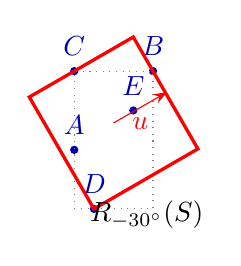
\begin{tikzpicture}[>=Stealth]
  \coordinate (a) at (1,1);
  \coordinate (b) at (2,2);
  \coordinate (c) at (1,2);
  \coordinate (d) at (1.25,.25);
  \coordinate (e) at (1.75,1.5);
  \fill[blue!70!black] (a) circle (1.5pt) node[above=2pt] {$A$};
  \fill[blue!70!black] (b) circle (1.5pt) node[above=2pt] {$B$};
  \fill[blue!70!black] (c) circle (1.5pt) node[above=2pt] {$C$};
  \fill[blue!70!black] (d) circle (1.5pt) node[above=2pt] {$D$};
  \fill[blue!70!black] (e) circle (1.5pt) node[above=2pt] {$E$};

  \node[draw=gray,dotted,fit=(a)(b)(c)(d)(e),inner sep=0pt] {};
  \node[draw=red,very thick,rotate fit=30,fit=(a)(b)(c)(d)(e),inner sep=0pt] (r) {};
  \draw[red,->] (r.center) -- (r.east) node[midway,below] {$u$};
  \node[below=4pt] at (r.south) {$R_{-30^\circ}(S)$};
\end{tikzpicture}
\end{document}
